\chapter{Extended Dependency Analysis}\label{ch:loops}

Chapter \ref{sec:design} introduced the basic principles of the dependency analysis and how the results of the dependency analysis can be used to measure the amount of leaked information for a given program. In this chapter, we will extend the dependency analysis to include the handling of arrays and more complex control flow structures, such as loops and function calls.

\paragraph{Sequential Execution Value}
So far, we used the execution value $\llbracket p \rrbracket_h (v)$ to get the actual value of $v$ during the execution with input $h$. Allowing loops and function calls in our input programs means that it is possible for statements to be executed multiple times. A value $v$ can thereby have more than one execution value during an execution.
To ensure that the execution value of a value is still well defined, we add a parameter $i$ that signifies, which of the possible execution values we want to refer to.

\begin{definition}[Sequential Execution Value]
    For a program $p$ and an input value $h$, we define the sequential execution value function as
    \begin{center}
        $\llbracket p \rrbracket_h: \val_p \times \mathbb{N} \to \{0, 1\} ^w \cup \{\bot\}$.
    \end{center}
    For a value $v$, $\llbracket p \rrbracket_h(v, i)$ is the numerical value of the $i$-th assignment of $v$ during the execution. If there is no $i$-th assignment of the value, the function returns $\bot$.
\end{definition}

\paragraph{Execution Condition $exec(\cdot)$ in Loops}
In our analysis, we treat loops as if they were separate functions. Therefore, when computing the execution condition $exec(\cdot)$ for the basic blocks of a program, we need a special handling of the blocks inside a loop:

The execution condition for the loop header will be computed in the standard way.

For the blocks inside the loop, we assume they form a separate function with the loop header being the entry block. We compute the execution condition for those blocks in the standard way, but under the assumption that $exec(b) = \mttt$ for the loop header $b$.

Since we treat loops as a function rather than a control flow structure, we annotate the edge between the loop head $b$ and the block following the loop header after the loop $\hat{b}$ with $follow((b, \hat{b})) = \mttt$. The execution condition $exec(\hat{b})$ is computed using this annotation.

\section{Loops}\label{sec:loops}
Loops are handled during the dependency analysis with the following steps:

First, we isolate the loop from the rest of the program and analyze the loop body as a separate function. Second, we generate the dependency vectors for loop output values. These dependency vectors act as a map from the loop inputs to the loop outputs. We compute the outputs of specific iterations using this map. Finally, we combine the iteration results into dependency vectors that represent the effect of the loop during the execution as a whole.

Because all three steps refer to the same program values in a different context, we use different notations to differentiate between them. The notations represent the value as an element of $\val_p$ and are used as alternative names for the values during different stages of the analysis. For a program value $v$ that is defined inside a loop $l$:
\begin{itemize}
    \setlength\itemsep{0em}
    \item $v[l]$ is used instead of $v$ during the general loop body analysis, which is the analysis of the loop separate from the rest of the program.
    \item $v[l, i]$ refers to the value $v$ in the i-th iteration of the loop $l$.
    \item $v$ is the value $v$ in its state after the execution of the loop is finished
\end{itemize}

\begin{figure}
\begin{subfigure}{.5\textwidth}
    \centering
    \begin{algorithm}[H]
        \hspace*{\algorithmicindent} \textbf{Input} $\emptyset$ \\
        \hspace*{\algorithmicindent} \textbf{Output} $\mOut$: int
        \begin{algorithmic}[1]
        \State $\mOut: int \leftarrow 0$
        \State $j: int \leftarrow 1$
            \While{$j \neq 0$}
                \State $\mOut \leftarrow \mOut \: | \: j$
                \State $j \leftarrow j << 1$
            \EndWhile
    \end{algorithmic} 
    \end{algorithm}
    \caption{Program code before SSA-transformation}
    \label{fig:loop}
\end{subfigure}
\hfill
\begin{subfigure}{.4\textwidth}
    \centering
    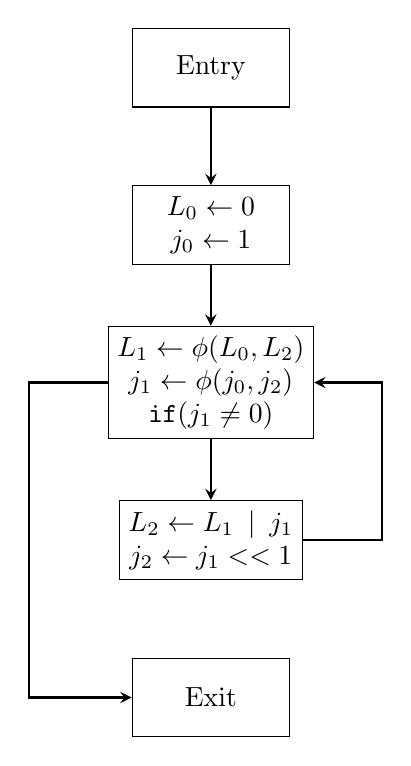
\begin{tikzpicture}
        \tikzstyle{node} = [rectangle, minimum width=2cm, minimum height=1cm, text centered, draw=black, node distance=2cm]
        \tikzstyle{arrow} = [thick,->,>=stealth]
                
                \node (entry) [node, xshift=1cm] {Entry};
                \node (b1) [node, below of=entry, align=center] {$L_0 \leftarrow 0$\\$j_0 \leftarrow 1$};
                \node (b2) [node, below of=b1, align=center] {$L_1 \leftarrow \phi(L_0, L_2)$ \\ $j_1 \leftarrow \phi(j_0, j_2)$\\ $\mathtt{if} (j_1 \neq 0)$};
                \node (b3) [node, below of=b2, align=center] {$L_2 \leftarrow L_1 \: \mid \: j_1$ \\ $j_2 \leftarrow j_1 << 1$};
                \node (exit) [node, below of=b3] {Exit};
                
                \draw[arrow] (entry) -- (b1);
                \draw[arrow] (b1) -- (b2);
                \draw[arrow] (b2) -- (b3);
                \draw[arrow] (b3.east) -- ++(1,0) |- (b2.east);
                \draw[arrow] (b2.west) -- ++(-1,0) |-(exit.west);
    \end{tikzpicture}
    \caption{CFG of the example program in SSA-form}
    \label{fig:whilegraph}
\end{subfigure}
\caption{Example program for Loop Analysis. The program doesn't have a secret input and always returns $111_2$.}\label{fig:loopEx}
\end{figure}

\paragraph{General Loop Body Analysis}
We begin the analysis by defining input and output values for a single loop iteration. 

The set of values that are used inside a loop can be divided into two categories:
\begin{enumerate}
    \item Values that might change with each iteration. These are values that are defined inside the loop (or before the loop in the case of the first loop iteration) and then get passed to the next iteration via a $\phi$-function in the loop header.
    \item Values that are constant for every loop iteration.
\end{enumerate}

The first group of values represents the inputs and outputs of a loop iteration, while the second group can be treated as constants in the loop analysis, even if their concrete value is unknown.

\begin{definition}[Loop Inputs and Outputs]
    Let $l$ be a loop in program $p$.
    \begin{itemize}
        \item[(a)] We define the set $in[l]$ of inputs of the loop as the set of values defined by $\phi$-functions in the header of the loop $l$.
        \item[(b)] We define the set $out[l]$ of outputs of the loop as the set of values that are defined inside the loop \emph{and} appear as arguments in a $\phi$-function in the loop header of $l$.
    \end{itemize}
\end{definition}

Analogous to the notation for values, $in[l]$ and $out[l]$ refer to the input and output sets during the general loop body analysis. The input and output sets for the $i$-th iteration are called $in[l, i]$ and $out[l, i]$.

Using the inputs and outputs, we can apply the principles of the basic dependency analysis to the loop $l$. We represent the values of the inputs as vectors of fresh boolean variables by setting $dVec(v[l]) = \var(v[l])$ for $v[l] \in in[l]$. Next, we compute the dependency vectors of all values defined inside the loop. 

The dependency vectors of the loop outputs $out[l]$ are made up of formulas that depend on
\begin{enumerate}
    \setlength\itemsep{0em}
    \item Variables that represent loop input bits
    \item Variables that represent program input bits
    \item Variables that represent loop input bits from enclosing loops
\end{enumerate}

Additional to the inputs and outputs, we define a propositional formula $exit[l]$ for the loop $l$, which represents the condition that must be fulfilled to jump out of the loop. Like the formulas for values in $out[l]$, $exit[l]$ depends on variables from the loop inputs, the program inputs, and enclosing loop inputs. 

\paragraph{Example}
Figure \ref{fig:loopEx} shows an example of a program containing a loop $l$. The inputs of the loop are the values $L_1[l]$ and $j_1[l]$. The outputs of the loop are the values $L_2[l]$ and $j_2[l]$.

The dependency vectors of those values are:
\begin{align*}
    dVec(L_1[l]) &= [L_1^2, L_1^1, L_1^0] \\
    dVec(j_1[l]) &= [j_1^2, j_1^1, j_1^0] \\
    dVec(L_2[l]) &= [L_1^2 \lor j_1^2, L_1^1 \lor j_1^1, L_1^0 \lor j_1^0] \\
    dVec(j_2[l]) &= [j_1^1, j_1^0, 0] \\
\end{align*}

The loop condition is $exit[l] = \left( [j_1^2, j_1^1, j_1^0] == [0, 0, 0] \right)$.

\paragraph{Computing Iterations}
We use the dependency vectors from the general loop body analysis, to obtain dependency vectors that represent the loop outputs after a specific iteration. The formulas in these vectors will then only depend on the program input variables and not the loop variables.

Input and output values of specific loop iterations are collected in the sets $in[l, i]$ and $out[l, i]$, where $i$ is the iteration count. The special case $i = 0$ refers to the program state before the loop is entered. We leave $in[l, 0]$ undefined and use $out[l, i]$ as the values that are computed before the loop and then used inside the loop during the first iteration. For $i > 0$ we have $in[l, i + 1] = out[l, i]$.

Given the dependency vectors for values in $in[l, i]$ for some value of $i$, we can compute the dependency vectors for values in $out[l, i]$, by substituting the variables representing values in $in[l]$ by the corresponding formula of the value in $in[l, i]$.

\begin{definition}[Iteration Substitution]
    Let $p$ be a program with a loop starting at block $l$. We are given dependency vectors for values in $in[l, i]$. To compute the dependency vectors for values in $out[l, i]$, we use the substitution
    \begin{center}
        $\sigma_{l, i} := \{h[l]^j \mapsto dVec(h[l, i])^j | \quad h[l] \in in[l]\}$
    \end{center}
    and apply it to the dependency vectors of $out[l]$.
\end{definition}

The substitution $\sigma_{l, i}$ can be applied to $exit[l]$ to obtain a formula $exit[l, i]$ that represents the condition of whether the loop is exited after the i-th loop iteration.

\paragraph{Example (cont'd)} The dependency vectors of the input and output values, as well as the loop condition, for the first iterations for the example program are presented in table \ref{tab:loop}. The construction of the substitution for $i = 1$ is shown below:

\begin{align*}
dVec(L_1[l]) &&:= [ && L_1^2 && L_1^1 && L_1^0 && ]\\
dVec(L_1[l, 0]) &&:= [ && 0 && 0 && 0 && ]\\
\sigma_{l, 1, L} && := \{ && L_1^2 \mapsto 0 && L_1^2 \mapsto 0 && L_1^0 \mapsto 0 && \} \\[1em]
dVec(j_1[l]) &&:= [ && j_1^2 && j_1^1 && j_1^0 && ]\\
dVec(j_1[l, 0]) &&:= [ && 0 && 0 && 1 && ]\\
\sigma_{l, 1, i} && := \{ && j_1^2 \mapsto 0 && j_1^2 \mapsto 0 && j_1^0 \mapsto 1 && \} \\[1em]
\sigma_{l, 1} && := &&\sigma_{l, 1, L} \cup \sigma_{l, 1, i}
\end{align*}

The dependency vectors for the values $j_2[l, 1]$ and $L_2[l, 1]$ are the result of applying the substitution $\sigma_{l, 1}$ to the vectors $dVec(j_2[l])$ and $dVec(L_2[l])$.

\begin{table}
    \centering
    \begin{tabular}{|c|c|c|c|c|c|}
    Iteration & \multicolumn{2}{|c|}{Inputs} & \multicolumn{2}{|c|}{Outputs} & Exit Condition \\
     & $L_1[l, i]$ & $j_1[l, i]$ & $L_2[l, i]$ & $j_2[l, i]$ & $exit[l, i]$ \\
     \hline
     $i = 0$ & - & - & $[0 0 0]$ & $[0 0 1]$ & $[001] == [000]$ \\
     $i = 1$ & $[0 0 0]$ & $[0 0 1]$ & $[0 0 1]$ & $[0 1 0]$ & $[010] == [000]$ \\
     $i = 2$ & $[0 0 1]$ & $[0 1 0]$ & $[0 1 1]$ & $[1 0 0]$ & $[100] == [000]$ \\
     $i = 3$ & $[0 1 1]$ & $[1 0 0]$ & $[1 1 1]$ & $[0 0 0]$ & $[000] == [000]$ \\
    \end{tabular}
    \caption{Dependency Vectors for the values of the sets $in[l, i]$ and $out[l, i]$ for the example program \ref{fig:whilegraph}.}
    \label{tab:loop}
\end{table}

\paragraph{Combining Iterations for Overall Loop Result}
To complete the loop analysis, we compute dependency vectors for the output values, that represent the loop execution as a whole.

The result values of the loop depend on the number of iterations that are executed. The case that the loop is executed exactly $i$ times is represented by the condition $iterations[l, i]$:

\begin{definition}[Loop Iterations]
    Let $p$ be a program with a loop beginning with basic block $l$.
    The propositional formula
    \begin{center}
        $iterations[l, i]: \left( \bigwedge\limits_{0 \leq j < i} \lnot exit[l, i] \right) \land exit[l, i]$
    \end{center}
    is a propositional formula that evaluates to true, iff for a program input $h$ the loop is executed exactly $i$ times. IT contains variables from $\var_p$ and variables representing inputs from enclosing loops where applicable.
\end{definition}

The formula $iterations[l, i]$ encodes the following intuition: For every $j < i$, \\$exit[l, j]$ must be false, otherwise the loop execution would have been aborted before the $i$-th iteration. The condition $exit[l, i])$ must be true, otherwise, the loop would have been executed more than $i$ times.

For the loop output values, we make the following observations:

We can check whether the loop is executed exactly $i$ times or not via the condition $iterations[l, i]$. If the loop is executed exactly $i$ times, the results are then equal to the outputs $out[l, i]$.  Continuing this observation for more iterations, leads to the definition of algorithm \ref{alg:loop}that computes the dependency vector for a loop output value. To ensure the termination of the algorithm, we have to limit the number of loop iterations it computes to an upper bound $maxIter$. The following paragraph discusses the soundness of this approximation.
\begin{figure}
    \centering
    \begin{algorithm}[H]
    \hspace*{\algorithmicindent} \textbf{Input} Iteration results $v[l, i]$ for the loop output value $v$ and \\
    \hspace*{\algorithmicindent} iteration conditions $iterations[l, i]$ \\
    \hspace*{\algorithmicindent} \textbf{Output} $dVec(v):$ Dependency vector that represents the overall computation result\\
    \hspace*{\algorithmicindent} \hspace*{\algorithmicindent}of the loop for the value $v$. \\
    
    \begin{algorithmic}[1]
        \State $dVec(v) \leftarrow \bot$ // initialize with placeholder value
        \State $i: int \leftarrow 0$
        \While{$i < maxIter$}
            \State $dVec(v) \leftarrow dVec(v).replace(\bot, \mathbb{IF}(iterations[l, i], \: dVec(v[l, i]), \bot))$
            \State $i++$
        \EndWhile
        \end{algorithmic}
\caption{Loop Result Computation}\label{alg:loop}
\end{algorithm}
    \caption{Algorithm for the computation of loop output values. The function \texttt{o.replace(x, y))} replaces occurrences of \texttt{x} in expression \texttt{o} with \texttt{y}}
\end{figure}


\paragraph{Approximation: Limiting Loop Iterations}\label{sec:approx}
Limiting the number of loop iterations means, that we exclude certain program inputs $h$ from the analysis, namely those that require more than $maxIter$ iterations. If such an input is used to evaluate the dependency vector of a loop output value $v$, $dVec(v)$ will evaluate to $\bot$. We interpret $\bot$ as an invalid execution and disregard the value in the following analysis. If the dependency vector $dVec(v) = \bot$ is used in the computation of the dependency vector for another value $v'$, $dVec(v')$ will also be set to $\bot$.

The exclusion of certain input values means, we have to adjust the equivalence from theorem \ref{thm:equiv}:

\begin{theorem}[Weakened Equivalence Theorem]\label{thm:weak}
    Given a program $p$, a program input value $h$ and a program value $v$ that is defined outside any loops. The dependency vector of the value $v$ fulfills the following condition:
    \begin{center}
        $\mathcal{V}_h(dVec(v)) \neq \bot \implies ( \forall 0 \leq i < w: \mathcal{V}_h(dVec(v)^i) \iff \llbracket p \rrbracket_h (v)^i)$
    \end{center}
\end{theorem}

Let $p$ be a program that contains a loop. We consider an execution that produces the output value $l$.
To compute the dynamic leakage of the execution and the channel capacity, we must adjust the method from section \ref{sec:leak} to take into account the weakened equivalence theorem.

\paragraph{Dynamic Leakage}
Any input value $h$ for which $\mathcal{V}_h(dVec(\mOut))$ doesn't evaluate to $\bot$ still fulfills theorem \ref{thm:equiv}. That means we can correctly decide if $h \in \mathcal{H}_l$. If we have an input value $h'$ for which $\mathcal{V}_{h'}(dVec(\mOut)) = \bot$, our analysis is not able to decide whether $h' \in \mathcal{H}_l$. However, we can safely approximate the set $\mathcal{H}_l$, by not adding any inputs with invalid executions to $\mathcal{H}_l$. Under-approximation is sound, because the knowledge gained by the attacker increases as the size of $\mathcal{H}_l$ decreases. Therefore the approximated dynamic leakage is a safe upper bound for the information leaked by the execution.

\paragraph{Channel Capacity}
The channel capacity analysis tries to find all possible outputs $l$. If we restrict the set $\mathcal{H}$ from which the inputs are taken, we possibly also restrict the set of possible outputs $\mathcal{L}$. To safely approximate the size of the set $\mathcal{L}$, we must assume that every input $h$ with $\mathcal{V}_h(dVec(\mOut)) = \bot$ produces a distinct output $l$ that is not the result of any other program execution. Over-estimating the size of $\mathcal{L}$ means over-estimating the amount of information an attacker might gain and is therefore sound.


\paragraph{Example (cont'd)}
Applying algorithm \ref{alg:loop} to the value $L_2$ from example \ref{fig:whilegraph}, gives the following results:
\begin{center}
\begin{align*}
    dVec(L_2) && = && \mathbb{IF}(([001] == [000]), && [000], \\
        && && \mathbb{IF}(([010] == [000]), && [001], \\
        && && \mathbb{IF}(([100] == [000]), && [011], \\
        && && \mathbb{IF}(([000] == [000]), && [111], \quad \bot)))) && \\[1em]
        && = && \mathbb{IF}((\mfff), && [000], \\
        && && \mathbb{IF}((\mfff), && [001], \\
        && && \mathbb{IF}((\mfff), && [011], \\
        && && \mathbb{IF}((\mttt), && [111], \quad \bot)))) && \\[1em]
        && = && && [111]
    \end{align*}
\end{center}

\section{Functions}\label{sec:functions}
We assume that all functions that are part of the input program are pure, i.e. they have no side effects. This means, the only way for information to flow into and out of the function is through the input parameters and the return value.

We write $\func$ for the set of functions that belong to a program $p$. For the analysis of the function $f$, we treat $f$ as its own program, where the parameters correspond to the input $\mIn$ and the return value corresponds to the output $\mOut$.

\paragraph{Function Analysis}
In the following, we first consider the analysis of non-recursive functions with a single return statement. Independent of any call sites of the function, we use the standard dependency analysis algorithm to compute dependency vectors for all values inside the function.

The dependency vectors computed for values of this function are defined over the variables created to represent the function's parameters. They do not contain variables representing bits of values from outside the function.

\paragraph{Dependency Analysis for \texttt{call}-Statements}
The statement $v \leftarrow \mathtt{call} \: f(a)$ calls the function $f$ with the arguments $a := (a_0,..., a_m)$ and assigns the return value of the call to the value $v$. To compute the dependency vector $dVec(v)$, we substitute the variables in $\var_f$ with the dependency vectors of the arguments:

\begin{definition}[Call Site Substitution]\label{def:callsiteSub}
    Let $f \in \func$ be a function in $p$ that has input parameters $\mathtt{P} := (\mathtt{P}_0,...,\mathtt{P}_m)$ and return value $r_f$ and let the expression $\mathtt{call} \: f(a)$ be a call to $f$ with the arguments $a := (a_0,..., a_m)$.
    
    The substitution $\sigma_{f(a)}$, defined as
    \begin{center}
        $\sigma_{f(a)} := \{ dVec(\mathtt{P}_i)^j \mapsto dVec(a_i)^j \: |  \: \mathtt{P}_i \in \mathtt{P}\}$
    \end{center}
    is called the \emph{call site substitution} of the expr $\mathtt{call} \: f(a)$ and substitutes the variables in $dVec(\mathtt{P}_i)$ representing the input parameters $\mathtt{P}_i$ by the corresponding boolean predicates of the dependency vectors belonging to the call site's arguments (note that $dVec(P_i)$ contains only variables that represent the bits of the function parameter $P_i$).
    
    The definition of $\mathcal{E}: \expr \to \mbform$ for function call expressions is then given as:
    \begin{center}
        $\mathcal{E}(\mathtt{call} f(a)) := \sigma_{f(a)} (dVec(r_f))$
    \end{center}
\end{definition}

\begin{lemma}
Using the extended definition of $\mathcal{E}$ including call-expressions, theorem \ref{thm:equiv} (theorem \ref{thm:weak} in case of loop approximation) is still fulfilled.
\end{lemma}

\section{Functions with Multiple Return Statements}\label{sec:multRet}

A function $f$ may have more than one return statement. Those statements in general return different values $v_1, ... v_k$. Thus it is necessary to combine the dependency vectors of these values into a single vector $r_f$ that accurately represents the returned value based on the arguments of this function. We assume that return statements are not contained in a loop.

The combining of multiple return values requires the following observation: If $b_1, b_2 \in \: \mbb_f$ are basic blocks that each contain a return statement and $b_1 \neq b_2$, then $exec(b_1) \land exec(b_2)$ is unsatisfiable. If this were not true, and $exec(b_1) \land exec(b_2)$ was satisfiable, then lemma \ref{lemma:exec} tells us, that there must be a set of function arguments for f, for which both $b_1$ and $b_2$ are executed. This would mean the execution of $f$ has multiple return values, which is an obvious contradiction. Thus, $exec(b_1) \land exec(b_2)$ must be unsatisfiable.

It follows directly from this observation that if a function has $k$ return statements which appear in the blocks $b_1, ..., b_k$, at most one of the conditions $exec(b_1),..., exec(b_k)$ can be fulfilled for any truth assignment. Simultaneously, every execution of a function with a return value includes a return statement. Hence exactly of the conditions $exec(b_1),... exec(b_k)$ must be fulfilled for any truth assignment.

Let $v_1, ... v_k$ be the values that are possibly returned by a function. The return statements are located in $b_1, .., b_k$ respectively. We compute the vector $r_f$ in such a way that, if for a function argument $a$ the condition $\mathcal{V}_a(exec(b_i))$ is true, $\mathcal{V}_a(r_f)$ will be equivalent to $\mathcal{V}_a(dVec(v_i))$. We define the function $select: 2^{\textsc{Val}_f \times BB_f} \to \mbform^w$ that fulfills this condition:

\begin{definition}[Value Selection]
    Let $s = \{s_0, ..., s_k\} \in 2^{\textsc{Val}_f \times BB_f}$ be a set of tuples where $s_i = (v_i, b_i)$. We define
    \begin{center}
        $select: 2^{\textsc{Val}_f \times BB_f} \to \mbform^w$
        $select(s) = \begin{cases}
            dVec(v) & |s| = 1 \text{ and } s = {(v, b)} \\
            \mathbb{IF} \left( exec(b_i), dVec(v_i), select(s \setminus s_i) \right) & |s| > 1, s_i = (v_i, b_i) \in s \text{ arbitrary}
        \end{cases}$
    \end{center}
    $select(s)$ corresponds to a sequential application of $\mathbb{IF}(\cdot, \cdot, \cdot)$
\end{definition}

\paragraph{Example}
Figure \ref{fig:mmult} shows a program that contains a function with three return statements. The possible return values in the example program are $0$ in block $b_1$, $1$ in block $b_3$ and $2$ in block $b_4$. The dependency vectors and execution conditions for the function \textsc{isEvenGreaterZero()} are:

\begin{align*}
    dVec(x) &&= && [x^2 x^1 x^0] \\
    dVec(0) &&= && [000] \\
    dVec(1) &&= && [001] \\
    dVec(2) &&= && [010] \\[1em]
    exec(b_1) &&= && x^2 \iff \mathtt{false} \\
    exec(b_3) &&= && x^2 \centernot\iff \mathtt{false} &&\land && x^0 \iff \mathtt{false} \\
    exec(b_4) &&= && x^2 \centernot\iff \mathtt{false} &&\land && x^0 \centernot\iff \mathtt{false}
\end{align*}

The return vector of the function \textsc{isEvenGreaterZero()} is given by:

\begin{align*}
    select({(0, b_1), (1, b_2), (2, b_3)}) && = \mathbb{IF}(exec(b_1), 0, && select({(1, b_2), (2, b_3)}) && \\
     && = \mathbb{IF}(exec(b_1), 0, && \mathbb{IF}(exec(b_2), 1, && select({(2, b_3)})) \\
      && = \mathbb{IF}(exec(b_1), 0, && \mathbb{IF}(exec(b_2), 1, && 2) \\
\end{align*}


\begin{figure}
\centering
    \begin{subfigure}{.7\textwidth}
    \begin{algorithm}[H]
        \hspace*{\algorithmicindent} \textbf{Input} $\mIn: int$ \\
        \hspace*{\algorithmicindent} \textbf{Output} $\mOut: int$\\
        \begin{algorithmic}[1]
            \State $\mOut \leftarrow $ \textsc{isEvenGreaterZero}$(\mIn)$
            \vspace{1em}
            \Procedure{isEvenGreaterZero}{$x: int$}: int
            \If{$x < 0$}
                \State \Return 0 
                \Else
                \If{$x \: \% \: 2 ==  0$}
                \State \Return 1
                \Else
                \State \Return 2
                \EndIf
            \EndIf
            \EndProcedure
        \end{algorithmic} 
    \end{algorithm}
    \caption{Source code of the example}
    \end{subfigure}
    
     \begin{subfigure}{.7\textwidth}
     \centering
       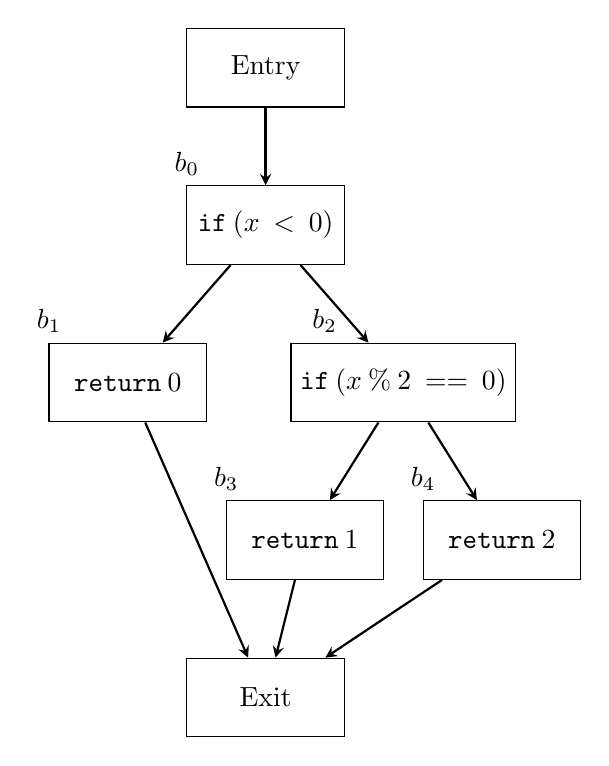
\begin{tikzpicture}
           \tikzstyle{node} = [rectangle, minimum width=2cm, minimum height=1cm, text centered, draw=black, node distance=2cm]
            \tikzstyle{arrow} = [thick,->,>=stealth]
            
            \node (entry) [node] {Entry};
            \node (b4) [node, below of=entry, label={[xshift=-1cm]$b_0$}] {$\mathtt{if} \: (x \: < \: 0)$};
            \node (b3) [node, below of=b4, xshift=-1.75cm, label={[xshift=-1cm]$b_1$}] {$\mathtt{return} \: 0$};
            \node (b1)  [node, below of=b4, xshift=1.75cm, label={[xshift=-1cm]$b_2$}] {$\mathtt{if} \: (x \: \% \: 2 \: == \: 0)$};
            \node (b2)  [node, below of=b1, xshift=1.25cm, label={[xshift=-1cm]$b_4$}] {$\mathtt{return} \: 2$};
             \node (b5)  [node, below of=b1, xshift=-1.25cm, label={[xshift=-1cm]$b_3$}] {$\mathtt{return} \: 1$};
            
            \node (exit) [node, below of=b5, xshift=-.5cm] {Exit};
            
            \draw[arrow] (entry) -- (b4);
            \draw[arrow] (b4) -- (b3);
            \draw[arrow] (b4) -- (b1);
            \draw[arrow] (b1) -- (b2);
            \draw[arrow] (b1) -- (b5);
            \draw[arrow] (b3) -- (exit);
            \draw[arrow] (b5) -- (exit);
            \draw[arrow] (b2) -- (exit);
       \end{tikzpicture}
       \caption{CFG for the function \textsc{isEvenGreaterZero}$(\cdot)$}
    \end{subfigure}
    \caption{Example program containing a function with multiple return statements}\label{fig:mmult}
\end{figure}


\section{Recursion}
We restrict the analysis of recursive functions in this section to functions that contain at most one recursive call. The analysis we present can be extended to functions with an arbitrary number of recursive calls.

To analyze recursive functions, we begin by applying the standard function analysis described in \ref{sec:functions} and \ref{sec:multRet}. However, call statements that recursively invoke the function that they are part of, are not handled in the standard way. Instead, we use placeholder variables $\rec := [\rec^{w - 1}, \rec^{w - 2}, ..., \rec^0]$ as the return value of the call.

\iffalse
\begin{figure}
\centering
    \begin{subfigure}{.5\textwidth}
        \centering
    \begin{algorithm}[H]
        \hspace*{\algorithmicindent} \textbf{Input} $\mIn: int$ \\
        \hspace*{\algorithmicindent} \textbf{Output} $\mOut: int$\\
        \begin{algorithmic}[1]
            \State $\mOut \leftarrow $ \textsc{sumRec}$(\mIn, 0)$
            \vspace{1em}
            \Procedure{sumRec}{$x: int, \: y: int$}: int
            \If{$x == 0$}
                \State $z_0: int \leftarrow y$ 
                \Else
                \State $z_1: int \leftarrow$ \textsc{sumRec}$(x - 1, y + 1)$
            \EndIf
            \State $z_2 \leftarrow \phi(z_0, z_1)$
            \State \Return $z_2$
            \EndProcedure
        \end{algorithmic} 
    \end{algorithm}
    \caption{A program containing a recursive function. The recursive function takes two arguments and adds their values together.}\label{fig:rec}
    \end{subfigure}
    \hfill
    \begin{subfigure}{.45\textwidth}
    \centering
        \begin{align*}
    dVec(x) := & [x^2 x^1 x^0] \\
    dVec(y) := & [y^2 y^1 x^0] \\
    dVec(z_0) := & [y^2 y^1 y^0] \\
    dVec(z_1) := & \bot \\
    dVec(z_2) := & \mathbb{IF}([x^2 x^1 x^0] == [000]), \\
    & \: [y^2 y^1 y^0], \: \bot)
\end{align*}
    \caption{Dependency vectors for the values in \textsc{sumRec}$(\cdot, \cdot)$}
    \end{subfigure}
    \caption{Example demonstrating the analysis of recursive functions}\label{fig:rec}
\end{figure}
\fi

\paragraph{Simulating Recursive Calls}
The analysis of a recursive function $f$ yields a dependency vector for the return value $r_f$ of $f$, which depends on the variables representing the input bits and contains placeholder variables from the vector $\rec$. These variables represent the return value $r_f$ of the recursive call inside the function.

Under our assumption that all program executions terminate, the vector $dVec(r_f)$ will not contain variables from $\rec$ for at least one function argument. If this wasn't the case, then there would be no way to end the recursion during the execution.

For notation, we use $r_f[i]$ to mean the value $r_f$ after the function $f$ was executed with a maximum recursion depth $i$. The return value we have computed so far is $r_f[0]$. We analyse recursive calls up until a recursion bound $recBound$ and write $r_f$ for $r_f[recBound]$.

To simulate the information flow of the recursive function call in the function $f$, we replace the placeholder value $\rec$ with $\sigma_{f(a)}(dVec(r_f))$, where $\sigma_{f(a)}$ is the call site substitution defined in \ref{def:callsiteSub} for the recursive call of $f$ with arguments $a$. The result vector of the replacement operation represents the execution of function $f$ including one recursive call and the placeholder value $\rec$ for any further recursive calls.

To simulate more than one recursive call, we repeat the same replacement operation until we reach a predefined recursion bound $recBound$. The algorithm to compute the final dependency vector of the return value of a recursive function is shown in figure \ref{alg:rec}.

\begin{figure}
    \centering
    \begin{algorithm}[H]
    \hspace*{\algorithmicindent} \textbf{Input} $dVec(r_f[0]):$ Dependency vector of $f$'s return value, \\
    \hspace*{\algorithmicindent} \hspace*{\algorithmicindent} containing $\rec$ as a placeholder.\\
    \hspace*{\algorithmicindent} \hspace*{\algorithmicindent} $\sigma_f(a): $Call site substitution for recursive call $\mathtt{call} f(a)$ \\
    \hspace*{\algorithmicindent} \textbf{Output} $dVec(r_f):$ Dependency vector of $f$'s return value.\\
    
    \begin{algorithmic}[1]
        \State $i: int \leftarrow 0$
        \While{$i < recBound$}
            \State $dVec(r_f[i + 1]) \leftarrow dVec(r_f[i]).replace(\rec, \: \sigma_{f(a)}(dVec(r_f[0])))$
            \State $i++$
        \EndWhile
        \end{algorithmic}
\caption{Recursive Function Return Value Computation}
\end{algorithm}
    \caption{Algorithm for the computation of return values of recursive functions. The function \texttt{o.replace(x, y))} replaces the elements of the vector \texttt{x} in expression \texttt{o} with the elements of the vector \texttt{y} that have the same index.}\label{alg:rec}
\end{figure}

\paragraph{Approximation: Limiting Recursion Depth}
By limiting the recursion depth to $recBound$, we may exclude inputs $h \in \mathcal{H}$ from the analysis, if the execution of $p$ with input $h$ requires more than $recBound$ recursive calls. The effects of this approximation on the computation of the information leakage of $p$ are the same as for the approximation in the loop analysis described in \ref{sec:approx}. We treat the approximations of the dynamic leakage and the channel capacity in the same manner as in the approximation for loop iterations.

\section{Break-Statements}
To analyze loops that contain break statements, the loop analysis from section \ref{sec:loops} has to be adapted at two points:
\begin{enumerate}
    \item Which values act as the output values of the loop now depends on the point at which the loop is exited: At the end of the loop body or at a break point?
    \item When the loop is exited is now also determined by whether or not a break statement is executed.
\end{enumerate}

\begin{figure}
\begin{subfigure}{.5\textwidth}
    \centering
    \begin{algorithm}[H]
        \hspace*{\algorithmicindent} \textbf{Input} $\mIn: int$ \\
        \hspace*{\algorithmicindent} \textbf{Output} $\mOut$: int
        \begin{algorithmic}[1]
        \State $\mOut: int \leftarrow 0$
        \State $j: int \leftarrow 1$
            \While{$j \neq 0$}
                \State $\mOut \leftarrow \mOut \: | \: j$
                \If{$\mIn < 0$}
                    \State \textbf{break}
                \EndIf
                \State $j \leftarrow j << 1$
            \EndWhile
    \end{algorithmic} 
    \end{algorithm}
    \caption{Program code before SSA-transformation}\label{prog:break}
\end{subfigure}
\hfill
\begin{subfigure}{.4\textwidth}
    \centering
    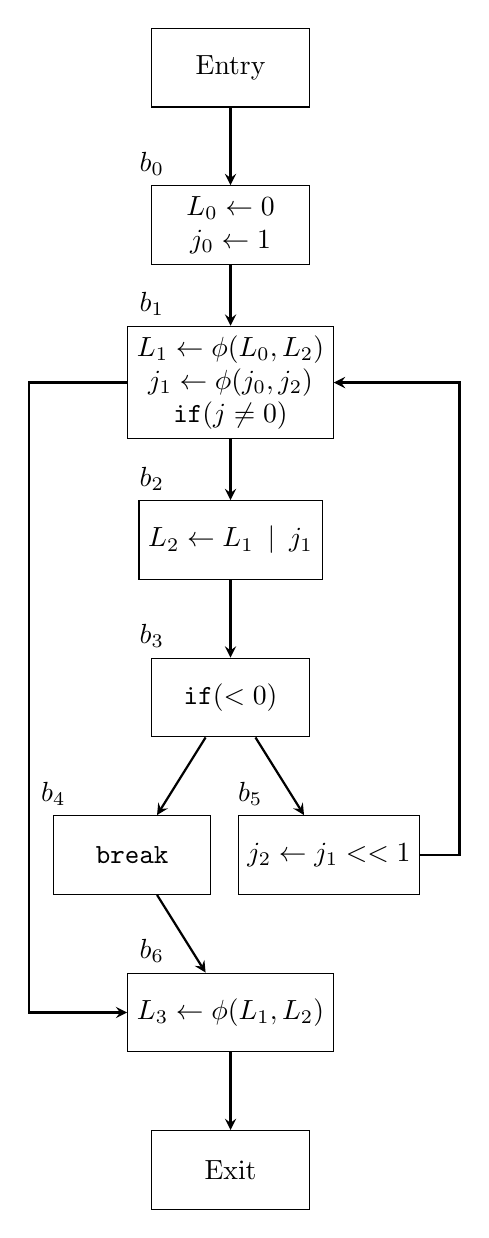
\begin{tikzpicture}
        \tikzstyle{node} = [rectangle, minimum width=2cm, minimum height=1cm, text centered, draw=black, node distance=2cm]
        \tikzstyle{arrow} = [thick,->,>=stealth]
                
                \node (entry) [node, xshift=1cm] {Entry};
                \node (b1) [node, below of=entry, align=center, label={[xshift=-1cm]$b_0$}] {$L_0 \leftarrow 0$\\$j_0 \leftarrow 1$};
                \node (b2) [node, below of=b1, align=center, label={[xshift=-1cm]$b_1$}] {$L_1 \leftarrow \phi(L_0, L_2)$ \\ $j_1 \leftarrow \phi(j_0, j_2)$\\ $\mathtt{if} (j \neq 0)$};
                \node (b21) [node, below of=b2, label={[xshift=-1cm]$b_2$}] {$L_2 \leftarrow L_1 \: \mid \: j_1$};
                \node (b22) [node, below of=b21, , label={[xshift=-1cm]$b_3$}] {$\mathtt{if} (\mIn < 0)$};
                \node (b23) [node, below of=b22, xshift=-1.25cm, label={[xshift=-1cm]$b_4$}] {\texttt{break}};
                \node (b3) [node, below of=b22, xshift=1.25cm, label={[xshift=-1cm]$b_5$}] {$j_2 \leftarrow j_1 << 1$};
                 \node (b31) [node, below of=b3, xshift=-1.25cm, label={[xshift=-1cm]$b_6$}] {$L_3 \leftarrow \phi(L_1, L_2)$};
                \node (exit) [node, below of=b31] {Exit};
                
                \draw[arrow] (entry) -- (b1);
                \draw[arrow] (b1) -- (b2);
                \draw[arrow] (b2) -- (b21);
                \draw[arrow] (b21) -- (b22);
                \draw[arrow] (b22) -- (b23);
                \draw[arrow] (b22) -- (b3);
                \draw[arrow] (b3.east) -- ++(.5,0) |- (b2.east);
                \draw[arrow] (b2.west) -- ++(-1.25,0) |-(b31.west);
                \draw[arrow] (b31) -- (exit);
                \draw[arrow] (b23) -- (b31);
    \end{tikzpicture}
    \caption{CFG of the example program}\label{fig:breakcfg}
\end{subfigure}
\caption{Example program for Loop Analysis. The program returns $001_2$ if $\mIn < 0$, otherwise $111_2$.}\label{fig:break}
\end{figure}

\paragraph{Loop Output Values}
The identification of the loop output values happens during the general loop body analysis, where we analyze the loop body independent of the rest of the program. The goal is to identify values, that represent the output of a single loop iteration. We continue to use the notations from section \ref{sec:loops}.

Previously we identified the output values of a loop by analyzing the arguments of the $\phi$-functions inside the loop header. For every input value, an output value is identified. The input value is mapped to this output value. The mapping represents the execution of the loop. When the loop contains a break statement, the output value depends on whether the execution of the loop body is completed or exited early via a break statement.

Let $v[l]$ be an input value to a loop. If the loop is without break statements we can map $v[l]$ to a single loop output value $v'[l]$. If the loop does contain break statements, we first collect the set of possible output values for $v[l]$: For each location, the loop could be exited at, the set contains the value that $v'[l]$ should be mapped to, if the exit is taken. This value can be found by analyzing whether the block following the loop exit contains a $\phi$-function for this value and if yes, which arguments the $\phi$-function has.

If no $\phi$-function is present, the output value at this point is the same as the input value of the loop. If a $\phi$-function is present, the output value at this point is the argument that belongs to the control flow of the basic block containing the break statement.

After having collected all possible output values for a loop input value, we combine the dependency vectors of those values into a single propositional vector that represents the overall output value for the aforementioned input value. The method for combining the dependency vectors is the same as for the combination of return values during the function analysis. When applying the $select(\cdot)$ function, we arrange the values in such a way, that this output value is chosen iff all execution conditions of the break blocks evaluate to false.

\paragraph{Example}
An example program containing a \texttt{break}-statement is given in figure \ref{fig:break}. The loop in the example program has the input values $L_1$ and $j_1$. For each of those, there are two possible output values: one value for exiting the loop via the break statement and one value for exiting the loop normally. For the value $L_1$ both of those output values are equal. $L_1$ is mapped to the output value $L_2$. The input value $j_1$ is mapped to itself, if the loop is exited via the \texttt{break} and to $j_2$ otherwise.

The execution condition $exec(b_4)$ of the block containing the break is given by $exec(b_4) := \mIn < 0$. Not that the execution conditions for blocks inside a loop are computed separately from the rest of the program.

The propositional vectors for the output values of the loop are finally given by:
\begin{align*}
    \text{Output value for input $L_1$:} && \mathbb{IF}(\mIn < 0 , L_2 , L_2) && = && L_2 \\
    \text{Output value for input $j_1$:} && \mathbb{IF}(\mIn < 0 , j_1, j_2)\\
\end{align*}

\paragraph{Exiting the Loop}
A loop that contains break statements is exited if the loop condition in the header is unfulfilled or if a break statement is executed. A break statement is executed if the condition $exec(b)$ for the block $b$ that contains the break statement is fulfilled. If $b_0, ..., b_k$ are all blocks in the loop that contain a break statement, the loop is exited if $exit[l] \lor \left(\bigvee\limits_{0 \leq i \leq k} exec(b_i)\right)$ is fulfilled. This extended exit condition replaces the simple exit condition $exit[l]$ during the loop analysis.

\section{Arrays}
The analysis can support fixed-size arrays with value semantics. For fixed-size arrays, the length must be known at compile time.

Before the dependency analysis begins, arrays are turned into a set of values that each represent an array element. The values have to be transformed into SSA-form. New array value copies are introduced at the instantiation of the array as well at every \texttt{write} instruction. Even though a \texttt{write} only modifies a single array element, we generate new value copies for all array elements. This is necessary, because in general, it is not possible to know which array element is modified.

For notation, we use superscript indices ($a^0, a^1, ...$) for the values representing the elements of the array $a$. Subscript indices ($a^0_0, a^0_1,...$) indicate the copies of those variables created during the SSA transformation.

The new values represent array entries for which we compute dependency vectors that describe the execution value of the array entry, analogous to the other values.

\paragraph{Array Instantiation}
If a new array is instantiated, all values are initialized with \texttt{0}. Their dependency vectors are constant vectors containing the value $\mfff$.

\paragraph{Array Write}
Consider the expression $a[k] \leftarrow e$, where we write the result of the expression $e$ to the k-th element of the array $a$. Let $a$ be an array of length $m$. The values for the array entries before the write instruction are called $a_i^0, a_i^1,..., a_i^{m-1}$ and the values for the array entries after the write instruction are called $a_{i+1}^0, a_{i+1}^1,..., a_{i+1}^{m-1}$.

The dependency vectors of the values $a_{i+1}^0, a_{i+1}^1,..., a_{i+1}^{m-1}$ are given by:
\begin{center}
    $dVec(a_{i+1}^j) := \mathbb{IF}(j == k, \mathcal{E}(e), a_i^j), \quad i = 0...m-1$
\end{center}
The expression assigns the array entry value the propositional vector $\mathcal{E}(e)$, if the index $j$ of the entry corresponds to the write-index $k$. Otherwise, the array entry is not changed.

\paragraph{Array Read}
Consider the expression $v \leftarrow a[i]$, where we assign the value of the i-th element of the array $a$ to the value $v$.
Let $a := [a^0, ..., a^m]$ be the array entry values that represent the array $a$ at the read instruction.

We define a function $choose(\cdot, \cdot): \: \mathbb{N} \times 2^{\val_p} \to \val_p$ that accepts an integer $i$ and an ordered set $S$ of values as inputs and returns the $i$-th element of $S$. Using this function we define the dependency vector for the value $v$ as:
\begin{center}
    $dVec(v) := choose(i, a)$
 a\end{center}